\documentclass[../../layout.tex]{subfiles}

\begin{document}
\chapter{Example chapter}
\blindtext[1]

\section{Using figures}
A Figura \ref{fig:rpi} é um exemplo. As referências
devem ser colocadas no arquivo .bib

\begin{figure}[H]
\centering
\caption{Raspberry Pi}
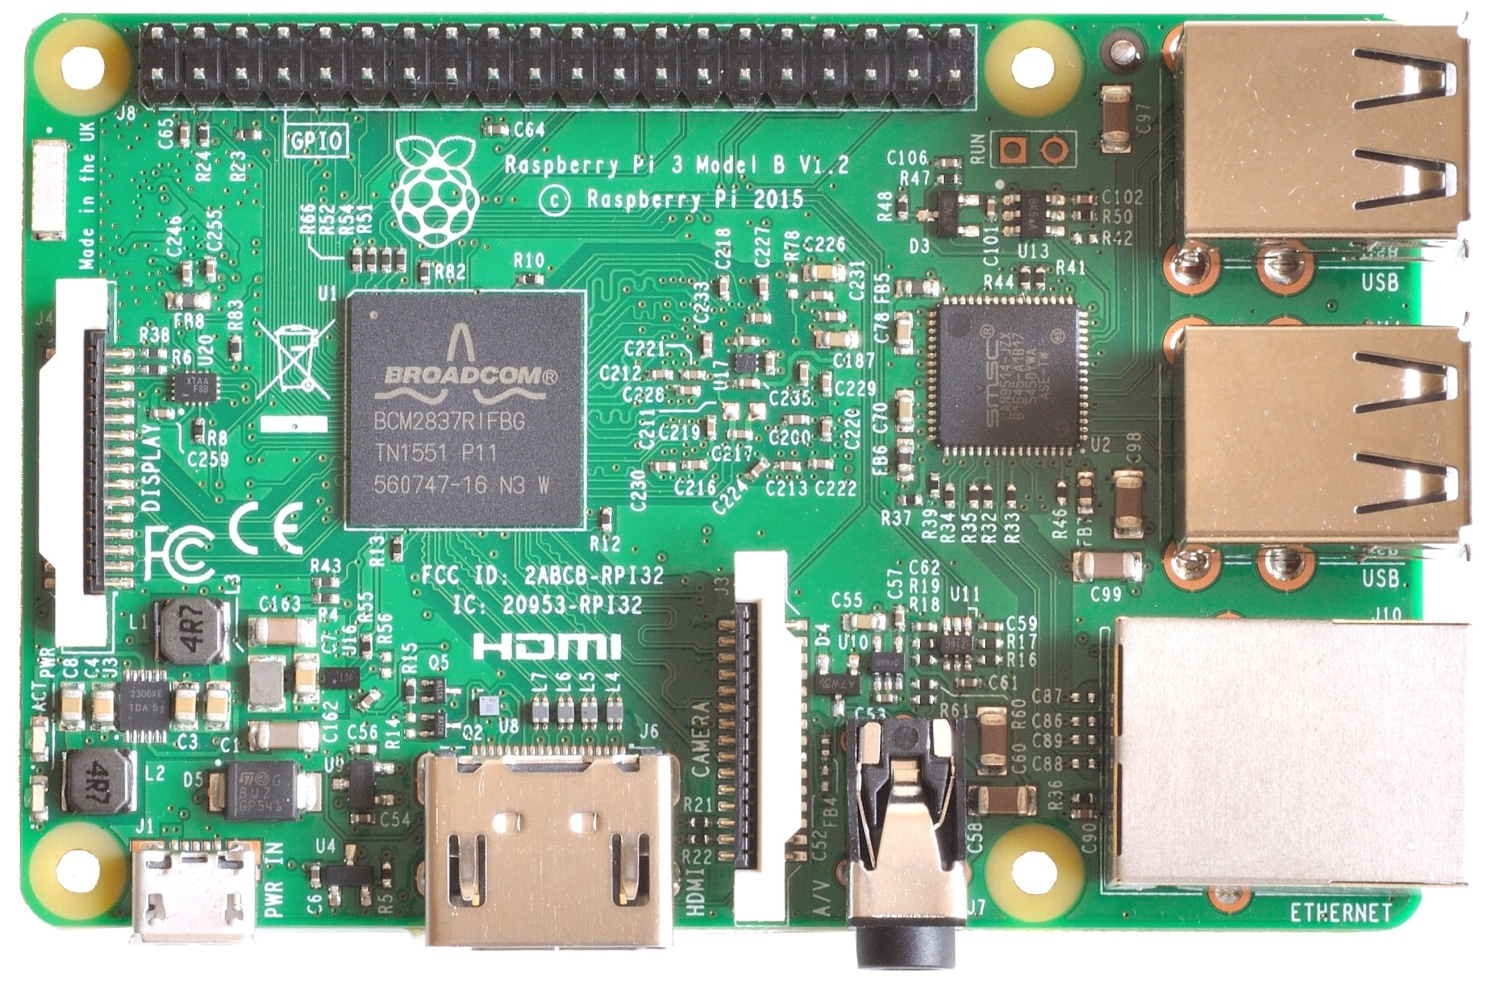
\includegraphics[width=0.5\textwidth]{assets/static/img/rpi.jpg}
\label{fig:rpi}

\begin{minipage}{0.5\textwidth}
\raggedright \footnotesize Fonte: Retirado de \acite{rpi}
\end{minipage}
\end{figure}

\section{Using code}
\blindtext[2]

\subsection{typed}
\begin{minted}{python}
import numpy as np
\end{minted}

\subsection{from file}

\begin{listing}[h]
\inputminted[
linenos,
tabsize=2,
frame=lines,
framesep=1em
]{ruby}{assets/code/example_code.ex}
\caption{Example from external file}
\label{listing:example}
\end{listing}

\end{document}
